\chapter{Implementation Verification using Ideal Membership Testing} \label{ch:date}

This chapter describes our approach to the problem of formal
verification of hardware implementations of arithmetic circuits over
finite fields of the type ${\mathbb{F}}_{2^k}$, using a
computer-algebra/algebraic-geometry based approach.  Given a
specification polynomial $f$ and a circuit $C$, we have to prove that
the circuit $C$ correctly implements $f$. Otherwise, we have to
generate a counter example that excites the bug in the design. 
The arithmetic circuit is modeled as a polynomial system in
${\mathbb{F}}_{2^k}[x_1,x_2,\cdots,x_d]$ and the verification problem
is formulated using Strong Nullstellensatz over finite fields as a
membership test in a corresponding (radical) ideal.   This requires
the computation of a Gr\"obner basis, which is computationally
expensive.  To overcome this limitation, we analyze 
the circuit topology and derive a term order to represent
the polynomials. Subsequently, using the theory of Gr\"obner bases
over finite fields, we prove that this term order renders the
set of polynomials itself a Gr\"obner basis of this (radical) ideal -- thus
significantly enhancing verification efficiency. Using our approach, we can
verify the correctness of, and detect bugs in, up to 163-bit circuits
in $\mathbb{F}_{2^{163}}$, corresponding to the NIST-specified ECC
standard.  In contrast, contemporary approaches, including SAT, SMT,
BDD, AIG based techniques, are infeasible. 

%%%%%%%%%%%%%%%%%%%%%%%%%%%%%%%%%%%%%%%%
%%%%%%%%%%%%%%%%%%%%%%%%%%%%%%%%%%%%%%%%
%%%%%%%%%%%%%%%%%%%%%%%%%%%%%%%%%%%%%%%%
\section{Problem Statement}
%Our objective is to address the problem of verifying correctness of a custom designed
%circuit implementation against a given word-level specification in cryptographic domain.
%The formal problem statement is given as follows:
The following is our problem statement:

\begin{itemize}
\item Given a finite field $\mathbb{F}_{2^k}$, i.e. given $k$
  (datapath size), along with the   corresponding irreducible
  polynomial $P(x)$. Let $P(\alpha) = 0$, i.e. $\alpha$ be the root of
  $P(x)$.   

\item Given a word-level specification polynomial $S =
  \mathcal{F}(A^{1},A^{2},\dots,A^{n}) \pmod{P(x)}$,  where each
  $A^{i}$ represents a word-level $k$-bit input; $S,
  A^{1},A^{2},\dots,A^{n} \in \mathbb{F}_{2^k}$;   $\mathcal{F}$ is a
  function describing the input-output relation.  

\item  Given a gate-level combinational circuit $C$. The bit-level
  primary inputs of the circuit are
  $\{a_{0}^{j},a_{1}^{j},\dots,a_{k-1}^{j}\}$, for $j=1,\dots, n$;
  the primary outputs are $\{z_0, \dots, z_{k-1}\} = Z$. Here $a_{i}^{j},
  z_i \in \mathbb{F}_2, i = 0, \dots, k-1$.  

\item   The word-level and bit-level correspondences are the following: \\
	$A^{1} = a_0^{1} + a_1^{1}\alpha + \dots +
        a_{k-1}^{1}\alpha^{k-1}=( a_{k-1}^{1}\cdots
        a_{1}^{1}a_{0}^{1})$,\\ 
	  $\vdots$ \\
      $A^{n} = a_0^{n} + a_1^{n}\alpha + \dots +
      a_{k-1}^{n}\alpha^{k-1}=( a_{k-1}^{n}\cdots
      a_{1}^{n}a_{0}^{n})$,\\ 
    and the primary outputs are related as:\\
     $Z = z_0 + z_1\alpha + z_2 \alpha^2 +\dots +
     z_{k-1}\alpha^{k-1}=( z_{k-1}\cdots z_{2}z_{1}z_{0})$.    
\end{itemize}
Our goal is to formally prove that $\forall A^{j}, Z \in
\mathbb{F}_{2^k}$, the circuit output $Z$ correctly implements the
specification $S = \mathcal{F}(A^{1},A^{2},\dots,A^{n}) \pmod{P(x)}$ 
 over $\mathbb{F}_{2^k}$. Otherwise, we have to produce a
 counter-example that excites the bug in the design.  

\begin{Example}
Consider the verification problem instance for a multiplier circuit
over $\mathbb{F}_{2^k}$. 
\begin{itemize}

\item Given the finite field $\mathbb{F}_{2^k}$ and the corresponding
  irreducible polynomial $P(x)$. Let $P(\alpha) = 0$.   

\item Given a word-level multiplier specification polynomial $S = A
  \cdot B \pmod{P(x)}$,  where $A, B, S \in \mathbb{F}_{2^k}$ ($k$-bit
  vectors). Function $\mathcal{F}$  corresponds to multiplication
  operation: $A\cdot B \pmod {P})$. 

\item  Given a gate-level combinational circuit. The bit-level primary
  inputs of the circuit are $\{a_0, \dots, a_{k-1}, ~b_0, 
  \dots, b_{k-1}\}$, and $\{z_0, \dots, z_{k-1}\}$ are the primary
    outputs; here $a_i, b_i, z_i \in \mathbb{F}_2, i = 0, \dots, k-1$. 
    Therefore, $A = a_0 + a_1\alpha + a_2\alpha^2 + \dots +    a_{k-1}\alpha^{k-1}$,
    $ B = b_0 + b_1 \alpha + b_2\alpha^2 + \dots +    b_{k-1}\alpha^{k-1}$ 
    and $Z = z_0 + z_1\alpha  + \dots +  z_{k-1}\alpha^{k-1}$.   
    
\end{itemize}
 We need to check whether the circuit implementation matches the
 specification, i.e., whether $S=Z, \forall a_{i},b_{i}$. 
	
\end{Example}

Our approach is generic enough to verify the implementation of any
combinational finite field arithmetic circuit against the given
polynomial specification. Without loss of generality and for the
purpose of exposition of our proposed approach, we use finite
field multiplier circuits for our verification objective, as they form
the core of most computations and are notoriously hard to verify. 

%%%%%%%%%%%%%%%%%%%%%%%%%%%%%%%%%%%%%%%%
%%%%%%%%%%%%%%%%%%%%%%%%%%%%%%%%%%%%%%%%
%%%%%%%%%%%%%%%%%%%%%%%%%%%%%%%%%%%%%%%%
\section{Verification Setup and Polynomial Modeling}
%using Polynomial System}
\label{sec:formulation}

%Traditional equivalence verification setup is first to set a miter circuit and then prove the miter is unsatisfiable.
%Instead, we setup the problem as an ideal membership testing: testing whether a given specification is a ``member" of the circuit.
%If the membership is established, then the circuit meets the specification. Otherwise, there must be bugs in the circuit design.

Our verification setup is depicted in Fig. \ref{fig:setup}. Given the
specification polynomial $S= A \cdot B \pmod{  P(x)}$,  and the
circuit implementation with $A,B$ as inputs and $Z$ as output, we want
to verify the property $S=Z$ over $\mathbb{F}_{2^k}$. 
%prove that for all possible inputs, $S$ is 
%always equal to $Z$ over $\mathbb{F}_{2^k}$.

%  If indeed there are no solutions
%to $F \neq G$, then it implies that $F$ is always equal to
%$G$. Otherwise, if there is a solution to our problem instance, then
%there is an assignment where $F$ differs from $G$ which indicates a
%bug in the implementation.    
  
\begin{figure}[b]

\centerline{
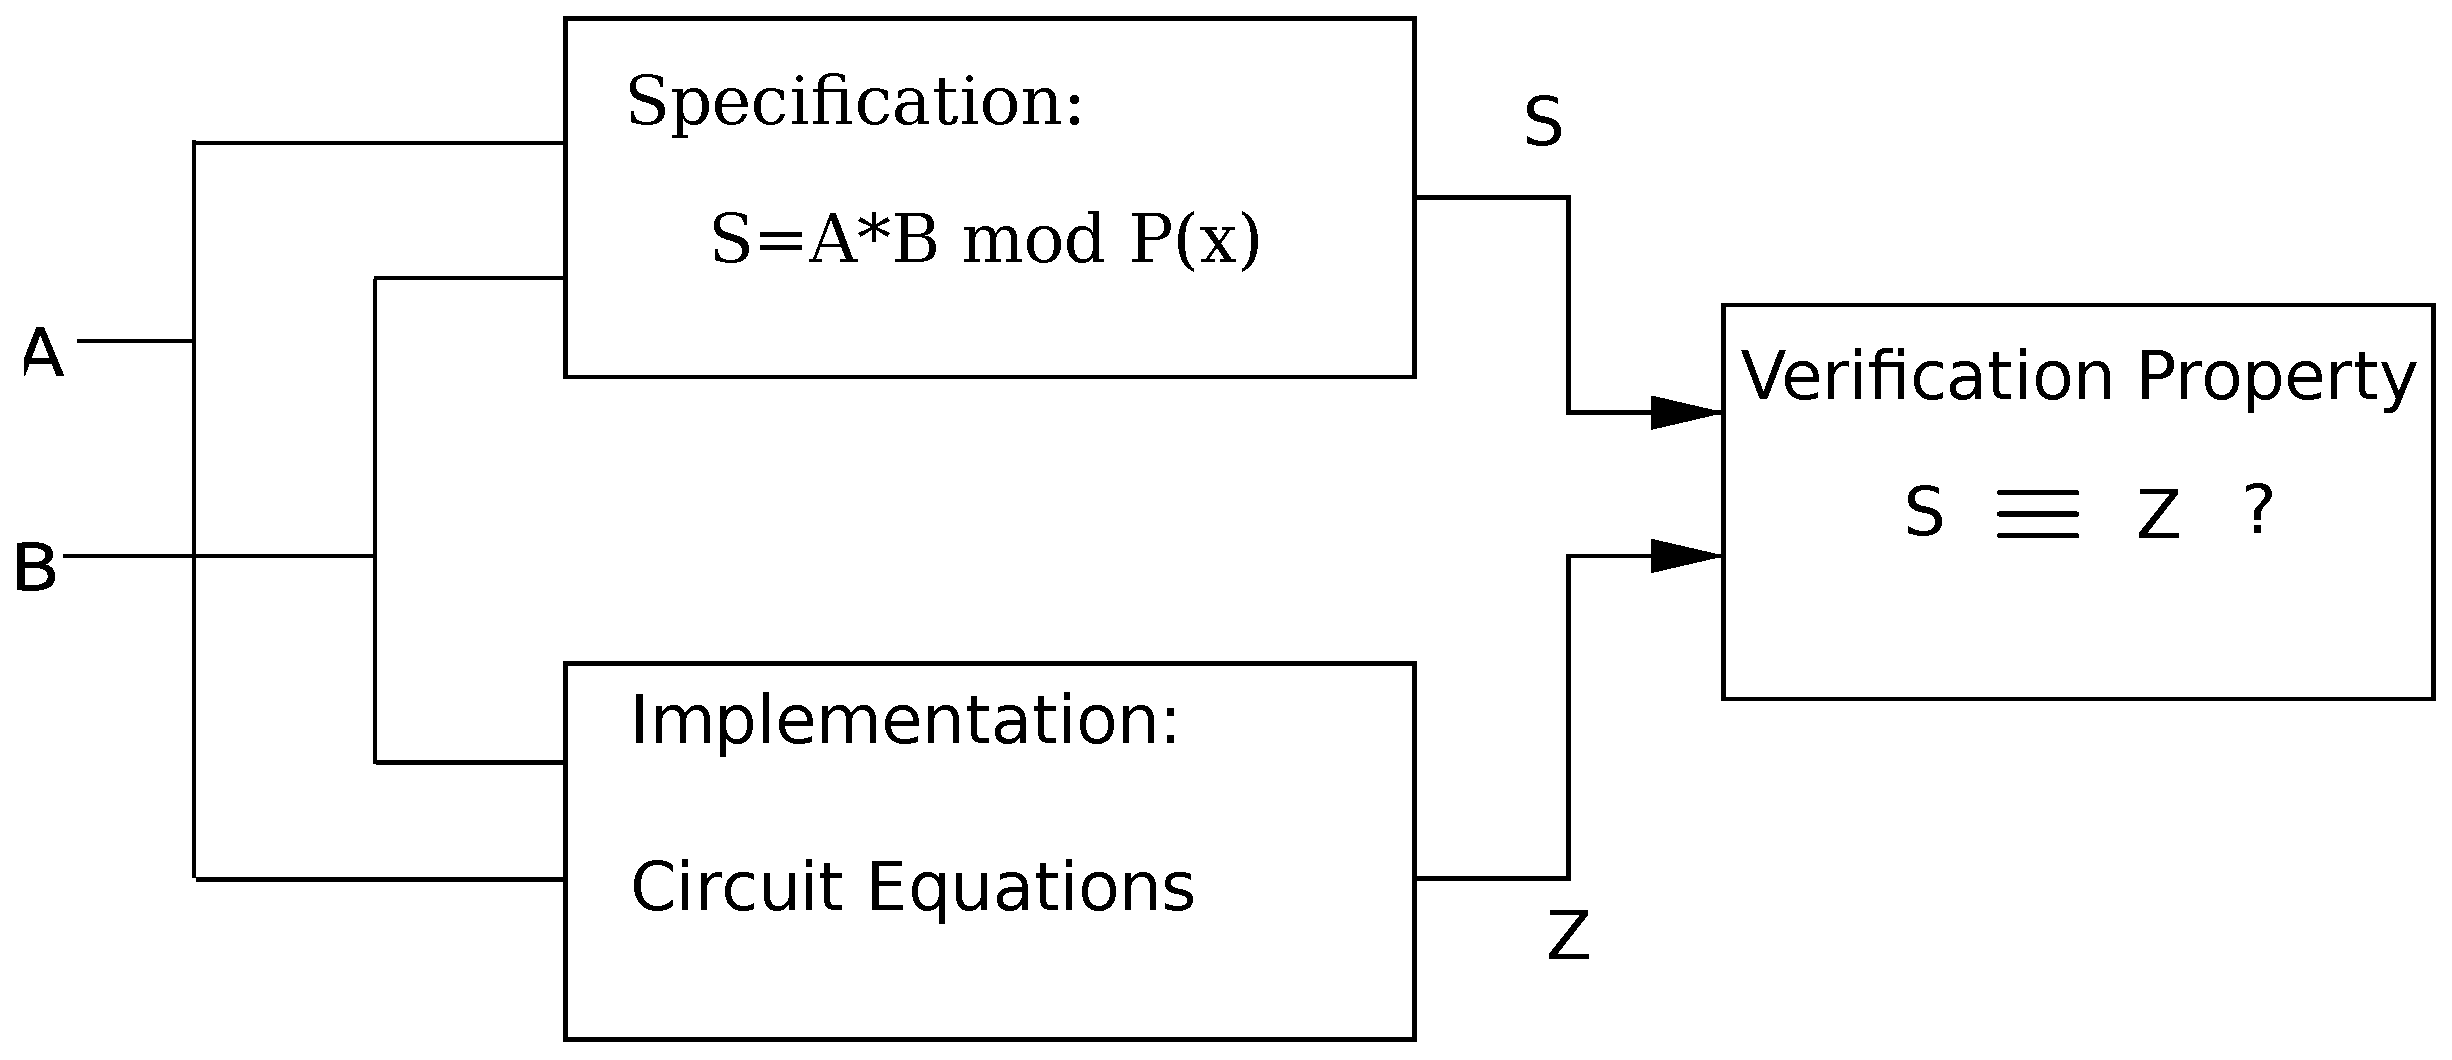
\includegraphics[scale=0.25]{./figures/setmember.eps}
}
\caption{The verification setup}
\label{fig:setup}
\end{figure}

{\bf Specification:} Given two $k$-bit inputs in bit-vector form
$A=(a_{k-1}a_{k-2}\cdots a_{1}a_{0})$ and $B=(b_{k-1}b_{k-2}\cdots
b_{1}b_{0})$, the specification can be modeled in polynomial forms in
$\mathbb{F}_{2^k}$ as follows: 

\begin{align}
A=&a_0+a_1\cdot \alpha+\cdots+a_{k-1}\cdot \alpha^{k-1} \nonumber \\
B=&b_0+b_1\cdot \alpha+\cdots+b_{k-1}\cdot \alpha^{k-1} \nonumber \\
S=&A\cdot B \pmod {P(x)} \nonumber
\end{align}

%where $A, B \in \mathbb{F}_{2^k} ~(a_i, b_i \in \mathbb{F}_{2})$ symbolically represent the inputs, 
%and $S\in \mathbb{F}_{2^k}$ represents the result of the multiplication. 

{\bf Implementation:} Given a gate-level circuit netlist, we map the gate-level
Boolean operators (AND, OR, NOT, XOR) to polynomials over
$\mathbb{F}_2 (\subset \mathbb{F}_{2^k})$ using the following
one-to-one mapping over $\mathbb{B} \rightarrow \mathbb{F}_2$ : 
\begin{equation}
\label{b2poly}
\begin{split}
\neg a\rightarrow a+1 \pmod 2  \\  
a \vee b \rightarrow a+b+a\cdot b \pmod 2  \\ 
a \wedge b \rightarrow a\cdot b \pmod 2  \\ 
a \oplus b \rightarrow a+b \pmod 2 
\end{split}
\end{equation}
where $a,b \in \mathbb{F}_{2}=\{0,1\}$.
Note that the equation $c=\mathcal{F}(a,b)$ is written in polynomial
form as $c-\mathcal{F}(a,b)=c+\mathcal{F}(a,b)$, ~as $-1 \equiv +1
\pmod 2$. 


 %a special mapping is the mapping of equation:
%\begin{equation}
%c=\mathcal{F}(a,b) \rightarrow c-\mathcal{F}(a,b)=0 \rightarrow c+\mathcal{F}(a,b)=0 \nonumber
%\end{equation}
%where $f$ represents any Boolean operator.

\begin{Example}
Consider the equation with Boolean operators: 
\begin{equation}
z=a \oplus (b \vee c). \nonumber
\end{equation}

The equation modeled over $\mathbb{F}_{2}$ is:
\begin{equation}
z+a + b + c + b\cdot c=0 \nonumber
\end{equation}  

The left-hand side expression is a polynomial in
$\mathbb{F}_{2}\left[a,b,c,z\right] \subset
\mathbb{F}_{2^{k}}\left[a,b,c,z\right]$: 
\begin{equation}
z+a + b + c + b\cdot c \nonumber
\end{equation}  
\end{Example}

Therefore, we can transform the entire circuit implementation as
polynomials over $\mathbb{F}_{2^k}$.  Let $Z$ symbolically denote the
word-level result of the implementation, i.e. the output of the
circuit.   

{\bf The Verification Property:}
The property $S=Z$ is modeled as a polynomial  $f: S+Z=0$ over
$\mathbb{F}_{2^k}$. 

Overall, our verification constraints can be modeled as a polynomial
system as follows:  

\begin{eqnarray}
 \left .  \begin{aligned}
f_1(x_1,x_2,\cdots, x_d)=0  \\
f_2(x_1,x_2,\cdots, x_d)=0  \\
\vdots  \\
%f_s(x_1,x_2,\cdots, x_d)=0  \\
f_{Z}: Z+z_{0}+z_{1}\cdot \alpha,\cdots,{z_{k-1}}\cdot \alpha^{k-1}=0   
 \end{aligned} 
\ \right\}
 &\qquad&  \text{\it Circuit implementation} \nonumber \\
 \left . \begin{aligned}
f_{A}:A+a_0+a_1\cdot \alpha+\cdots+a_{k-1}\cdot \alpha^{k-1}=0   \\ 
f_{B}:B+b_0+b_1\cdot \alpha+\cdots+b_{k-1}\cdot \alpha^{k-1}=0   \\ 
f_{spec}: S+A\cdot B =0   
 \end{aligned} 
\right\}
 &\qquad&  \text{\it Word-level specification} \nonumber \\
 \left .  \begin{aligned}
f:S+Z=0  \nonumber 
 \end{aligned} 
\right\}
 &\qquad& \text{Property:}~S = Z~?~
\end{eqnarray}


\begin{Example}
\label{exp:mul2bit}
Consider a 2-bit multiplier over ${\mathbb{F}}_{2^2}$ with
$P(x)=x^{2}+x+1$, given in Fig. \ref{fig:2bitmul}. Variables $a_0,
a_1, b_0, b_1$ are primary inputs, $z_0, z_1$ are primary outputs, and
$c_0, c_1, c_2, c_3, r_0$ are intermediate variables. The gate $\otimes$
corresponds to AND-gate, i.e. bit-level multiplication modulo 2. The
gate $\oplus$ corresponds to XOR-gate, i.e. addition modulo 2.

\begin{figure}[b]
\centerline{
\includegraphics[scale=0.5]{./figures/2bitmultiplier.eps}
}
\caption{ A 2-bit multiplier over ${\mathbb{F}}(2^2)$.}
\label{fig:2bitmul}
\end{figure}

The circuit can be described using the following Boolean equations:
\begin{align*}
c_0=a_0 \wedge b_0,   \nonumber \\
c_1=a_0 \wedge b_1,   \nonumber \\
c_2=a_1 \wedge b_0, \nonumber \\
c_3=a_1 \wedge b_1,   \nonumber \\
r_0=c_1 \oplus c_2 ,      \nonumber \\
z_0=c_0 \oplus c_3,   \nonumber \\
z_1=r_0 \oplus c_3,    \nonumber
\end{align*}

With the mapping rules given in Equation \ref{b2poly}, 
the above equations are transformed into the following polynomials:
\begin{align*}
c_0+a_0 \cdot b_0,   \nonumber \\
c_1+a_0 \cdot b_1,   \nonumber \\
c_2+a_1 \cdot b_0,   \nonumber \\
c_3+a_1 \cdot b_1,   \nonumber \\
r_0+c_1 + c_2 ,      \nonumber \\
z_0+c_0 + c_3,   \nonumber \\
z_1+r_0 + c_3,   \nonumber
\end{align*}

Therefore, our overall polynomial system is:
\begin{eqnarray}
 \left .  \begin{aligned}
f_1: c_0+a_0 \cdot b_0  \\
f_2: c_1+a_0 \cdot b_1  \\
f_3: c_2+a_1 \cdot b_0  \\
f_4: c_3+a_1 \cdot b_1  \\
f_5: r_0+c_1 + c_2		\\
f_6: z_0+c_0 + c_3		\\
f_7: z_1+r_0 + c_3		\\
f_{Z}: Z+z_0+z_1\cdot \alpha   
 \end{aligned} 
\ \right\}
 &\qquad&  {\text {\it Circuit constraints}} \nonumber \\
 \left . \begin{aligned}
f_{A}: A+a_0+a_1\cdot \alpha  \\ 
f_{B}: B+b_0+b_1\cdot  \alpha  \\ 
f_{spec}: S+A\cdot B   
 \end{aligned} 
\right\}
 &\qquad&  {\text {\it specification}} \nonumber \\
 \left .  \begin{aligned}
f: S+Z  \nonumber 
 \end{aligned} 
\right\}
 &\qquad& \text{\it Property to verify:} ~S = Z~? 
\end{eqnarray}

\end{Example}

%As shown above, our verification problem is clearly algebraic in nature. 
%Therefore, the use of polynomial algebra is most suitable for such applications.

With the polynomial model given above, we formulate our problem as 
{\bf (radical) ideal membership testing},  which is described next.


%%%%%%%%%%%%%%%%%%%%%%%%%%%%%%%%%%%%%
%%%%%%%%%%%%%%%%%%%%%%%%%%%%%%%%%%%%%
%%%%%%%%%%%%%%%%%%%%%%%%%%%%%%%%%%%%%%%%
\section{Verification Formulation as Ideal Membership Testing}\label{sec:radicaltest}

%Given a specification polynomial $f: S + A\cdot B$ where $A =
%a_0 + a_1 \alpha + \dots + a_{k-1}\alpha^{k-1}, B = b_0 + b_1 \alpha +
%\dots + b_{k-1}\alpha^{k-1}$. 
%We are also given a gate-level circuit $Z$ with
%$\{a_0, \dots, a_{k-1}, ~b_0, \dots, b_{k-1}\}$ as primary inputs and
%$\{z_0, \dots, z_{k-1}\}$ as the primary outputs. We have to check if
%the circuit $Z$ implements the function $f$ over the given field
%$\mathbb{F}_{2^k}$. 

To formulate our verification test, we first analyze the circuit and
model the Boolean gate-level operators as polynomials over
$\mathbb{F}_2 ~(\subset \mathbb{F}_{2^k})$, as given by the
mappings of Equations \ref{b2poly}.  
To this set we then append the polynomials corresponding to the
word-level specification.  Let $\{f_1,f_2,\ldots,f_s\}$ denote this
set of polynomials derived from  both {\it specification} and {\it
  implementation}.  
%$A + a_0 + a_1\alpha + \dots + a_{k-1}\alpha^{k-1}$, 
%$B + b_0 + b_1\alpha + \dots b_{k-1}\alpha^{k-1}$, 
%$Z + z_0 + z_1 \alpha + \dots + z_{k-1}\alpha^{k-1}$; 
%these polynomials specify the correspondence between the bit-level ($\mathbb{F}_2$) 
%and the word-level ($\mathbb{F}_{2^k}$) variables in the system. 
%We denote these constraints as polynomials $\{f_1, \dots, f_s\}$ over
%the ring $\mathbb{F}_{2^k}[x_1,\dots, x_d]$, 
Let $\{x_1,x_2,\ldots,x_d\}$ denote all the variables in the
polynomial system. As a consequence, $\{f_1,f_2,\ldots,f_s\}\in
\mathbb{F}_{2^k}[x_{1},\dots,x_{d}]$. Let $J = \langle f_1,
\dots,f_s\rangle \subset \mathbb{F}_{2^k}[x_{1},\dots,x_{d}]$ denote
the ideal generated by these polynomials. Our verification property
$S=Z$ is also modeled as a polynomial $f: S+Z \in
\mathbb{F}_{2^k}[x_{1},\dots,x_{d}]$. 
% (Note $S=G$ is not included)
%Let $\{x_1,x_2,\ldots,x_d\}$ denote all variables occurring in {\it specification} and {\it implementation}, where $x_i\in \mathbb{F}_2 \subset \mathbb{F}_{2^k}$.
%We denote the generated ideal as $J = \langle f_1, \dots,f_s\rangle$.  

To prove that the specification polynomial ($f$) matches the
implementation ($J = \langle f_1, \dots, f_s\rangle$), we need to
check whether $f: S+Z=0$  {\it agrees} with all the solutions of $J$
over the field $\mathbb{F}_{2^k}$. In computer algebra terminology, we
need to check {\it whether or not $f$ vanishes on the variety
  $V_{\mathbb{F}_{2^k}}(J)$},  where $V_{\mathbb{F}_{2^k}}(J)$ denotes
the variety of ideal $J$ over the given field $\mathbb{F}_{2^k}$.
This is because for all points (solutions) $p \in
V_{\mathbb{F}_{2^k}}(J)$, if $f(p) = 0$, then $f: S + Z = 0 \implies S
=Z$. On the other hand, if $f(p) \neq 0$ for some point $p$, then $p$
corresponds to the bug in the design.  

Now if $f$ vanishes on $V_{\mathbb{F}_{2^k}}(J)$, according to
Proposition \ref{pro:iofv},  we know that $f$ should be a member of
the radical ideal $I(V_{\mathbb{F}_{2^k}}(J))$.  Therefore, our
verification test can be modeled as membership testing of $f$ in the
(radical) ideal $I(V_{\mathbb{F}_{2^k}}(J))$. To solve this problem,
we need to first derive the generators of $I(V_{\mathbb{F}_{2^k}}(J))$ 
(note that we are only given the generators of $J$), and then perform
the ideal membership testing using the Gr\"obner basis algorithm.  

\subsection{Generating $I(V_{\mathbb{F}_{2^k}}(J))$}
Strong Nullstellensatz establishes correspondences between ideals and their radicals.
As given in Theorem \ref{thm:sns},  $I(V_{\overline {\mathbb{K}}}(J)) =\sqrt{J}$, where 
the variety $V$ is taken over the algebraically closed field
$\overline {\mathbb{K}}$. Finite fields are, however, {\it not}
algebraically closed, as shown by the following result from
\cite{galois_field:mceliece}:  

\begin{Theorem}
Given finite fields $\mathbb{F}_{2^n}$ and $\mathbb{F}_{2^m}$ such that $n$ divides
$m$. Then $\mathbb{F}_{2^n} \subset \mathbb{F}_{2^m}$.
\end{Theorem}

Therefore, $\mathbb{F}_2 \subset \mathbb{F}_{2^2} \subset
\mathbb{F}_{2^4} \subset \mathbb{F}_{2^8} \subset \dots$; and
$\mathbb{F}_2 \subset \mathbb{F}_{2^3} \subset \mathbb{F}_{2^6}  \dots
$; and so on. The algebraic closure of $\mathbb{F}_{2^k}$ is known to
be  an infinite field obtained as the union of all such finite fields.  


Therefore, Nullstellensatz needs to be suitably modified for
application over finite fields. 
%Let $\overline {\mathbb{F}_{2^k}}$ denote the algebraic closure of $\mathbb{F}_{2^k}$.
We re-visit the notion of vanishing polynomials for this purpose. 

Over the finite field $\mathbb{F}_{2^k}$, any element $A$ satisfies
the property $A^{2^k}-A=0$. Therefore, polynomial  $x^{2^k}-x$
vanishes at all points in $\mathbb{F}_{2^k}$, and $x^{2^k}-x$ is
called the vanishing polynomial of the field. As a consequence, the
variety $V(x^{2^k}-x)=\mathbb{F}_{2^k}$. Over multivariate polynomial
ring $\mathbb{F}_{2^k}[x_1,\dots,x_d]$,
$V(x_1^{2^k}-x_1,\dots,x_d^{2^k}-x_d)$ is $\mathbb{F}_{2^k}^d$. 
 
In the sequel, we use the following notation: 
Let $J_0=\langle x_1^{2^k}-x_1,\dots,x_d^{2^k}-x_d \rangle $ denote
the ideal of vanishing polynomials over $\mathbb{F}_{2^k}$. Also, if
$J=\langle f_1,\dots,f_s \rangle$ 
%and  $J_0=\langle x_1^{2^k}-x_1,\dots,x_d^{2^k}-x_d \rangle $, 
then the sum of ideals $J+J_0=\langle f_1,\dots,f_s ,
~~x_1^{2^k}-x_1,\dots,x_d^{2^k}-x_d \rangle$.  Let $\overline
{\mathbb{F}_{2^k}}$ denote the algebraic closure of
$\mathbb{F}_{2^k}$. 

\begin{Lemma} \label{lem:closure}
Let $J \subset \mathbb{F}_{2^k}[x_1,\dots,x_d]$ be any ideal and let
$J_0=\langle x_1^{2^k}-x_1,\dots,x_d^{2^k}-x_d \rangle$. Then
$V_{\mathbb{F}_{2^k}}(J)=V_{\overline {\mathbb{F}_{2^k}}}(J+J_0)$. 
\end{Lemma}

\begin{Proof}
 Since $\overline {\mathbb{F}_{2^k}} \supset \mathbb{F}_{2^k}$, we have :

\begin{eqnarray}
V_{\mathbb{F}_{2^k}}(J) &= & V_{\overline {\mathbb{F}_{2^k}}}(J) \cap \mathbb{F}_{2^k}^d  \nonumber \\
 		   &= & V_{\overline {\mathbb{F}_{2^k}}}(J) \cap  V_{\mathbb{F}_{2^k}}(J_0)  \nonumber \\
 		   &= &  V_{\overline {\mathbb{F}_{2^k}}}(J) \cap  V_{\overline{\mathbb{F}_{2^k}}}(J_0) \nonumber  \\
		   &= & V_{\overline {\mathbb{F}_{2^k}}}(J+J_0) \nonumber
\end{eqnarray}
\end{Proof}

As a consequence of the above lemma, variety of any ideal $J$ over a
finite field $\mathbb{F}_{2^k}$ can be equivalently  analyzed over its
algebraic closure $\overline {\mathbb{F}_{2^k}}$ by just appending to
$J$ all the vanishing polynomials $J_0$. These vanishing polynomials
do not change the zero-set of $J$ but allow the same analysis over the
algebraic closure. 

\begin{Lemma}\label{lem:selfrad}
$I(V_{\mathbb{F}_{2^k}}(J))=I(V_{\overline {\mathbb{F}_{2^k}}}(J+J_0))=\sqrt {J+J_0}$.
\end{Lemma}

\begin{Proof}
As shown above, $V_{\mathbb{F}_{2^k}}(J)=V_{\overline {\mathbb{F}_{2^k}}}(J+J_0)$.
Therefore, $I(V_{\mathbb{F}_{2^k}}(J))=I(V_{\overline {\mathbb{F}_{2^k}}}(J+J_0))$.
According to Strong Nullstellensatz, $I(V_{\overline
  {\mathbb{F}_{2^k}}}(J+J_0))=\sqrt {J+J_0}$. Thus: 
\begin{equation}
I(V_{\mathbb{F}_{2^k}}(J))=I(V_{\overline {\mathbb{F}_{2^k}}}(J+J_0))=\sqrt {J+J_0}
\end{equation}
\end{Proof}

\begin{Lemma}\label{lem:root}
Let $J$ be any arbitrary polynomial ideal in
$\mathbb{F}_{2^k}[x_1,\dots,x_d]$ and $J_0$ be the corresponding
vanishing ideal. Then $J+J_0$ is radical. In other words, $\sqrt
{J+J_0}=J+J_0$. 
\end{Lemma}
\begin{Proof}
This is a well known result, a proof of which is given in
\cite{gao:gf-gb-ms}. 
\end{Proof}

Putting together the above results, we finally arrive at the following
application of Nullstellensatz over finite fields.

%%%%%%%%%%%%%%%%strong nullstellensatz in finite field%%%%%%%%%%%%%
\begin{Theorem}\label{thm:snff}
$\left[\bf{Strong\  Nullstellensatz\ in\ Finite\ Fields}\right]$ Let
$J \subset \mathbb{F}_{2^k}[x_1, x_2, \cdots, x_n]$ be an ideal and
$J_0$ be the ideal of vanishing polynomials. Then, 
\begin{equation}
I(V_{\mathbb{F}_{2^k}}(J))=J+J_0=J+\langle x_1^{2^k}-x_1,x_2^{2^k}-x_2,\cdots, x_d^{2^k}-x_d\rangle
\end{equation}
\end{Theorem} 

\begin{Proof}
Combining Lemma \ref{lem:selfrad} and Lemma \ref{lem:root}, 
\begin{equation}
I(V_{\mathbb{F}_{2^k}}(J))=I(V_{\overline {\mathbb{F}_{2^k}}}(J+J_0))=\sqrt {J+J_0}=J+J_0
\end{equation}
where $J_0=\langle x_1^{2^k}-x_1,x_2^{2^k}-x_2,\cdots, x_d^{2^k}-x_d\rangle$.
\end{Proof}

{\bf Overall Verification Problem Formulation:} Through Strong
Nullstellensatz over finite fields, given an ideal $J$, we can
directly construct ideal $I(V_{\mathbb{F}_{2^k}}(J))=J+J_0$.  For our
verification problem, we take the polynomials $\{f_1, \dots, f_s\}$
representing the circuit constraints and the specification polynomials
to generate ideal $J$. Then we append the vanishing polynomials
$\{x_1^{2^k} - x_1, \dots, x_d^{2^k} - x_d\}$ of ideal $J_0$. Our
verification problem can now be formulated as testing whether the
verification property polynomial $f$ is in $J+J_0$. If $f \in (J +
J_0)$, correctness of the circuit is established. Otherwise, there is
a bug in the design. To test if $f \in (J + J_0)$, it is required to
compute a Gr\"obner  basis $G$ of the ideal $J+J_0$.  Then, we reduce
$f$ w.r.t. $G$: i.e., $f \stackrel{G}{\textstyle\longrightarrow}_+
r$. If $r=0$, then the circuit is correct, otherwise there is a bug in
the design.  


%Strong Nullstellensatz tells us $I(V(J)) =\sqrt{J}$. However, the result only 
%works over an algebraically closed field while finite fields are not an algebraically closed field.
%To solve this problem, an analogue in finite field $F_{2^k}$ of Strong Nullstellensatz is introduced here. 

%\begin{proof}
%Firstly, we need prove $J+\langle x_1^{2^k}-x_1,x_2^{2^k}-x_2,\cdots,x_d^{2^k}-x_d\rangle$ is radical. For convenience, let $q$ denote $2^k$, 
%let $I=J+\langle x_1^{2^k}-x_1,x_2^{2^k}-x_2,\cdots,x_d^{2^k}-x_d\rangle$.

%From Definition. \ref{def:radical}, we claim: 

%$f^m\in J \Rightarrow f\in J$, for some $m>0$.

%Let $I_0$ denoted $\langle x_i^q-x_i\rangle$. 
%Let $R$ denote $\mathbb{F}_q\left[x_1,x_2,\cdots,x_d\right]$.

%$\frac{R}{I_0}=\mathbb{F}_q\left[\overline x_i \mid {\overline x_i}^q=\overline x_i \right]$, 
%which means all variables have degree less than q in $\frac{R}{I_0}$.
%\begin{equation} \label{proofbasis}
%\forall g\in I_0\ \Leftrightarrow \ \bar{g}=0,\ where \bar{g}\in \frac{R}{I_0}.
%\end{equation}

%Let $g'=f^q-f$, where $f\in I$ .

%$\overline {f^q-f}=\overline {f^q}-\overline{f}$.

%$f\in I$ can be denoted as:
%\begin{equation}
%f=\displaystyle\sum\limits_{i=1}^n{a_i\cdot x_1^{i_1} \cdot x_2^{i_2} \cdots \cdot x_n^{i_n}}. \nonumber 
%\end{equation}

%then we can have the following two equations:
%\begin{equation}\label{fq}
%f^q=\displaystyle\sum\limits_{i=1}^n{a_i^q\cdot (x_1^q)^{i_1} \cdot (x_2^q)^{i_2} \cdots \cdot x_n^{i_n}}=\overline f. 
%\end{equation}
%\begin{equation}\label{fqbar}
%\overline {f^q}=\displaystyle\sum\limits_{i=1}^n{a_i^q\cdot (x_1^q)^{i_1} \cdot (x_2^q)^{i_2} \cdots \cdot x_n^{i_n}}. 
%\end{equation}

%From Eqn.\ref{fq} and Eqn.\ref{fqbar}, we can get
%\begin{equation}
%\overline {f^q}=\overline f \  \Leftrightarrow \ \overline {f^q}-\overline f=0 
%\end{equation}

%Then from Eqn.\ref{proofbasis}, we can have $f^q-f\ \in I_0 $, which then generates $(f^q-f)^q=f^{q^2}-f^q \in I_0$.

%\begin{equation}
 %\left.\begin{aligned}
        %f^q-f \in I_0 \\
        %f^{q^2}-f^q \in I_0
       %\end{aligned}
 %\right\}
 %\qquad  \Longrightarrow {f^{q^2}-f \in I_0} \nonumber
%\end{equation}

%Iteratively, we can have $\forall k\in\{0,1,2,\cdots\}, f^{q^k}-f\in I_0$.

%Then $\exists k',q^{k'} \ge m$, such that $f^m\in I \Rightarrow f^{q^k}\in I$.

%$f$ can be expressed as:

%$f=\underbrace{f-f^{q^k}}_{\in I_0 \subset I}+\underbrace{f^{q^k}}_{\in I}$.

%Now our claim is justified: if $f^m\in I$, then $f\in I$. In other words, $\sqrt{J+I_0}=J+I_0$.

%Secondly, we need prove $I(V(J))=J+I_0$.

%From Strong Nullstellensatz, we have:

%$I(V_{\overline {\mathbb{F}_q}}(J+I_0))=\sqrt{J+I_0}=J+I_0$.

%Notice $V_{\overline {\mathbb{F}_q}}(J+I_0)=V_{\mathbb{F}_q}(J)$.

%So we finally have $I(V_{\mathbb{F}_q}(J))=\sqrt{J+I_0}=J+I_0$. \hfill $\square$

%\end{proof}

%%%%%%%%%%%%%%%%%%%%%%%%%%%%%%%%%%%%%%%%%%%%%%%%%%%%%%%%%%%%

%Strong Nullstellensatz over $\mathbb{F}_{2^k}$ (Theorem \ref{thm:snff}) states this:
%\begin{equation}
 %I(V_{\mathbb{F}_{2^k}}(J)) = J + J_0 = \langle f_1, \dots, f_s, ~x_1^q-x_1, \dots, x_d^q - x_d\rangle. 
%\end{equation}
%Therefore, {\it we need to test whether or not $f$ is a member of the ideal $J + J_0$.}  


\begin{Example}
Let us re-consider Example \ref{exp:mul2bit}. First, polynomials are
extracted from the circuit implementation and the specification, as
shown in Example \ref{exp:mul2bit}. These polynomials represent the
ideal $J$. Along with the ideal $J_0=\langle x_1^{2^k}-x_1, \dots,
x_d^{2^k} - x_d \rangle$, the following polynomials represent $J+J_0$
for the multiplier circuit. 

\begin{eqnarray}
 \left .  
	\begin{aligned}
		f_1:c_0+a_0 \cdot b_0  \\
		f_2:c_1+a_0 \cdot b_1  \\
		f_3:c_2+a_1 \cdot b_0  \\
		f_4:c_3+a_1 \cdot b_1  \\
		f_5:r_0+c_1 + c_2		\\
		f_6:z_0+c_0 + c_3		\\
		f_7:z_1+r_0 + c_3		\\
		f_{Z}:Z+z_0+z_1\cdot \alpha   
	\end{aligned} 
 \ \right\}
 &\qquad&  {\it implementation ~(\subset J)} \nonumber \\
 \left . 
	\begin{aligned}
		f_{A}:A+a_0+a_1\cdot \alpha   \\ 
		f_{B}:B+b_0+b_1\cdot \alpha  \\ 
		f_{spec}:S+A\cdot B =0   
	\end{aligned} 
 \right\}
 &\qquad&  {\it specification ~(\subset J)} \nonumber \\
  \left . 
	\begin{aligned}
		a_0^2-a_0, ~a_1^2-a_1,~b_0^2-b_0, ~b_1^2-b_1   \\ 
		c_0^2-c_0, ~c_1^2-c_1,~c_2^2-c_2, ~c_3^2-c_3  \\ 
		r_0^2-r_0, ~z_0^2-z_0,~z_1^2-z_1    \\ 
		A^4-A, ~B^4-B ,~Z^4-Z,~ S^4-S		  
	\end{aligned} 
 \right\}
 &\qquad&  {\it \text{vanishing polynomials} (J_0)} \nonumber
\end{eqnarray}

Now we need to compute the Gr\"obner basis $G$ of this ideal
$J+J_0$. Once the computation of $G$ is completed, we simply need a
polynomial reduction to test whether $f: S+Z$ can be reduced by
$G$. In other words, we need test whether
$S+Z\stackrel{G}{\textstyle\longrightarrow}_+ 0$? 
\end{Example}



While our approach seems reasonably simple, the complexity of
Gr\"obner basis computation can make verification infeasible. 


%: first computing a Gr\"obner basis and then conducting a polynomial reduction. 
%Unfortunately, two problems regarding Gr\"obner basis computation arises: one is related to the complexity of Gr\"obner basis computation;
%the other one is related to the degree representation of vanishing polynomials.

%The Gr\"obner basis computation is known to have double-exponential worst-case complexity in the input data.
%Even over finite fields, the complexity still makes this approach impractical.

{\bf Complexity of Gr\"obner basis over finite fields:} For our
specific problem of computing a Gr\"obner basis for $J + J_0$ over
$\mathbb{F}_{q}$, the following result is known \cite{gao:gf-gb-ms}:

\begin{Theorem}\label{thm:gb-complexity}
Let $I = \langle f_1, \dots, f_s, ~x_1^q - x_1, \dots, x_d^q -
x_d\rangle \subset \mathbb{F}_{q}[x_1, \dots, x_d]$ be an ideal over
any finite field $\mathbb{F}_{q}$. The time and space complexity of
Buchberger's algorithm to compute a Gr\"obner basis of $I$ is bounded
by $q^{O(d)}$ assuming that the length of input $f_1, \dots, f_s$ is
dominated by $q^{O(d)}$.  
\end{Theorem}

In our case $q = 2^k$, and when $k$ and $d$ are large, this complexity
makes verification infeasible. 
%The second problem results from the degree representation of vanishing polynomials over large field. 
%Vanishing polynomials ($x_i^q - x_i$) introduce a practical problem. 
%Most computer algebra tools (Gr\"obner Bases engines) have a bound on the degree of variables in the system. 
%For our work, we use the {\sc Singular} \cite{DGPS} tool. 
%{\sc Singular} has a limitation that the degree of a variable ($q$ in $x^q$) be
%$<2^{16}$. In cryptography, one encounters very large fields $F_q$ where $q =
%2^{256}$ or higher. So we need to be able to find alternate ways to
%account for the high degree polynomials $x^q - x$ in $J_0$. 
%These two practical problems hinders the practical application of our approach.
%In subsequent sections, we offer our solutions to these problems.
In what follows, we show that a variable/term order can be derived by
analyzing the circuit topology which makes the set of polynomials
$\{f_1, \dots,f_s, x_1^{2^k} - x_1, \dots, x_d^{2^k} - x_d\}$ itself a
Gr\"obner basis of $J+J_0$ -- obviating the need to apply Buchberger's
algorithm. 

%%%%%%%%%%%%%%%%%%%%%%%%%%%%%%%%%%%%%%%%%%%%%%
%%%%%%%%%%%%  New Section  %%%%%%%%%%%%%%%%%%%
\section{Obviating Buchberger's Algorithm}
\label{sec:improv}

Just as variable orderings play a critical role in constructing BDDs
and solving SAT feasibly,  the Gr\"obner basis computation is also
highly susceptible to the term orderings imposed on the polynomials. 
Therefore a key step to improve/avoid the high complexity 
of Gr\"obner basis computation is to derive a ``good" term order.
%But unlike that there is no best variable order for SAT/BDD, there
%does exist an optimal variable order %for Gr\"obner basis computation
%in our case. With such an optimal variable order,  %the expensive
%computation of Gr\"obner basis can be obviated. 

Buchberger's work \cite{buchberger_thesis} initially laid the
foundation for computing Gr\"obner's bases.  Subsequently, many
improvements were introduced to improve the efficiency of Buchberger's
algorithm. Two of the most important improvements are the chain and
product criteria. For our particular circuit verification application,
we exploit the product criteria. 


\begin{Lemma}
\label{lemma:prodcriteria}
[Product Criterion \cite{productc:1979}] Let $\mathbb{F}$ be any
field, and $f, g \in \mathbb{F}[x_1,\cdots,x_d]$ be polynomials. If
the equality $lm(f) \cdot lm(g) = LCM(lm(f), lm(g))$ holds, then
$Spoly(f,g)\stackrel{G}{\textstyle\longrightarrow}_+ 0.$ 
\end{Lemma}

The above result states that when the leading monomials of $f, g$ are
relatively prime, then $Spoly(f, g)$ always reduces to 0 modulo $G$. Thus
$Spoly(f, g)$ need not be considered in Buchberger's algorithm. 
Modern computer algebra engines perform this check to avoid
unnecessary $Spoly(f, g)$ computations.  If we could analyze the given
circuit and  derive a term order such that every polynomial pair
($f,g$) in the generating set has relatively prime leading monomials,
then for all S-polynomials, the subsequent reduction would not add any
new polynomials in the basis. In other words, $Spoly(f, g)
\stackrel{G}{\textstyle\longrightarrow}_+ 0$ for all pairs $f,
g$. Consequently, the polynomials $\{f_1, \dots, f_s\}$ extracted from
the circuit (corresponding ideal $J$) and represented using such a
term order would itself constitute a Gr\"obner basis of $J$.  In
\cite{wienand:cav08}, the authors derive exactly such a term order,
and a similar concept can be applied in our case. 

Note that in our case: 
\begin{itemize}
\item since the circuit constraints $\{f_1, \dots,f_s\}$ are modeled
  as polynomials in $\mathbb{F}_2 \subset {\mathbb{F}}_{2^k}$,  they
  contain only multi-linear monomial terms;  
\item the output of a gate is uniquely computed, and it always appears
  as a ``single variable term'' in the 	polynomials; 
\item the circuit is acyclic;
\end{itemize}

Let $x_i$ be the output variable of any gate $H_i$ in the circuit, and
let $x_{p_1}, \dots,x_{p_j}$ denote variables that are the inputs to
the gate $H_i$.  If we can represent the polynomials $f_i$ such that
$x_i >$ every monomial  in the variables $x_{p_1}, \dots, x_{p_j}$,
then all $(f_i, f_j), i\neq j$ have  relatively prime leading
monomials and $\{f_1, \dots, f_s\}$ is a Gr\"obner basis. 
% (this is Proposition 2 in \cite{wienand:cav08}). 

\begin{Proposition} \label{prop:top-order}
Let $C$ be any arbitrary combinational circuit. Let $\{x_1, \dots,
x_d\}$ denote the set of all variables (signals) in the circuit,
i.e. the primary input, intermediate and primary output
variables. Perform a {\bf reverse topological traversal} of the
circuit and order the variables such that $x_i > x_j$ if $x_i$ appears
earlier in the reverse topological order. Impose a lex term order to
represent the Boolean expression for each gate as a polynomial $f_i$;
then $f_i = x_i + \text{tail}(f_i)$. Then the set of all polynomials
$\{f_1, \dots, f_s\}$ forms a Gr\"obner basis, as $lt(f_i)$ and $
lt(f_j)$ for $i\neq j$ are relatively prime. 
\end{Proposition}
	
\begin{Example}
Consider the circuit of Figure \ref{fig:2bitmul}, reproduced
below. Variables $a_0, a_1, b_0, b_1$ are primary inputs,  $z_0, z_1$
are primary outputs, and $c_0, c_1, c_2, c_3, r_0$ are intermediate
variables.   

\begin{figure}[htb]
\centerline{
\includegraphics[scale=0.4]{./figures/2bitmultiplier.eps}
}
\caption{ A 2-bit multiplier over ${\mathbb{F}}(2^2)$. The gate $\otimes$
corresponds to AND-gate, i.e. bit-level multiplication modulo 2. The
gate $\oplus$ corresponds to XOR-gate, i.e. addition modulo 2.}
\label{fig:mul2bit2nd}
\end{figure}

We perform a reverse topological traversal of the
circuit. Starting from the primary outputs, traverse the circuit 
to the primary inputs, and order the gates according to the their
(reverse) topological levels. The primary outputs $z_0,
z_1$ are both at level-0, variables $r_0, c_0, c_3$ are at
level-1, ~$c_1, c_2$ are at level-2, and the primary inputs
$a_0, a_1, b_0, b_1$ are at level-3. We order the variables $\{z_0 >
z_1\} > \{r_0 > c_0 > c_3\} > \{c_1 > c_2\} > \{a_0 > a_1 >  b_0 >
b_1\}$. Using this variable order, we impose a {\it lex} term order on
the monomials. Then the polynomials of $J$ all have relatively prime 
leading terms, as shown below: 

\begin{align*}
c_0+a_0 \cdot b_0, \ lm=c_0;  \nonumber \\
c_1+a_0 \cdot b_1, \ lm=c_1;  \nonumber \\
c_2+a_1 \cdot b_0, \ lm=c_2;  \nonumber \\
c_3+a_1 \cdot b_1, \ lm=c_3;  \nonumber \\
r_0+c_1 + s_2 , \ lm=r_0;     \nonumber \\
z_0+c_0 \cdot c_3, \ lm=z_0;  \nonumber \\
z_1+r_0 \cdot c_3, \ lm=z_1   \nonumber
\end{align*}


In our overall problem formulation, we also have variables $A, B, S, Z
\in \mathbb{F}_{2^k}$.  They can also be accommodated in this term
order by imposing $S >Z> A > B > z_0 > z_1 > r_0 > c_0 > c_3 > c_1 >
c_2 > a_0 > a_1 >b_0 > b_1$. 
\end{Example}

Thus, using the result of Proposition \ref{prop:top-order}, the set
of polynomials $\{f_1, \dots, f_s\}$ is a Gr\"obner basis for
$J$. Note that  $\{x_1^{2^k} - x_1, \dots, x_d^{2^k}
- x_d\}$ is a Gr\"obner basis for $J_0$. However, we have to compute a
Gr\"obner basis of $J + J_0 = \langle f_1, \dots, f_s, ~x_1^{2^k} - x_1,
\dots, x_d^{2^k} - x_d \rangle$.  Not all polynomials pairs in $\{f_1,
\dots, f_s, ~x_1^{2^k} - x_1, \dots, x_d^{2^k} - x_d\}$ have
relatively prime leading monomials.  

Consider an arbitrary polynomial $f_i \in J$. Using our term order, we
have $f_i = x_i + \text{tail}(f_i)$; i.e. the leading monomial of
$f_i$ is a single variable term $x_i$. Clearly, the pair
$(x_i+\text{tail}(f_i), ~x_i^{2^k}-x_i), ~f_i \in J, ~x_i^{2^k} - x_i \in J_0$
do not have relatively prime leading monomials. In fact, the pairs
$(x_i+\text{tail}(f_i), x_i^{2^k}-x_i)$ are the only ones to be considered
for Gr\"obner basis computation, as all other pairs have relatively
prime leading terms. This motivated us to investigate further the
question ``what is the result of the reduction
$\text{Spoly}(x_i+\text{tail}(f_i), x_i^{2^k}-x_i) 
\stackrel{J,J_0}{\longrightarrow}_+ r $?''. We state and prove the
following: 

\begin{Theorem}
\label{thm:contrib}
Let $q = 2^k$, and let $\mathbb{F}_q[x_1, \ldots, x_d]$ be a ring on
which we have a monomial order $>$. Let $I$ be a subset of $\{1,
\ldots, d\}$. For all $i \in I$, let $f_i = x_i +P_i$ (where $P_i =
\text{tail}(f_i)$) such that  all indeterminates $x_j$  that appear in
$P_i$ satisfy $x_i > x_j$.  Then the set $G = \{f_i :  i  \in I\} \cup
\{x_1^q-x_1, \ldots, x_d^q-x_d\}$ is a Gr\"obner basis.  
\end{Theorem}

\begin{Proof}
According to Buchberger's Theorem (Theorem 1.7.4 in \cite{gb_book}),
we need to show that for all $f, g \in G$, $Spoly(f,g)
\stackrel{G}{\rightarrow}_+ 0$. Let $G_1=\{ f_i : i \in I \}$. Lemma
\ref{lemma:prodcriteria} shows that if $f, g \in G$, have relatively
prime leading terms, then  $Spoly(f,g) \stackrel{G}{\rightarrow}_+
0$. So the only case where Lemma \ref{lemma:prodcriteria} does not
apply is when $f = x_i + P_i$ and $g = x_i^q-x_i$. Then $Spoly(f,g)=
x_i^{q-1} f - g = P_i x_i^{q-1} + x_i$. In what follows, it is important
to note that the indeterminates appearing in $P_i$ are all less than
$x_i$.  

First of all,  $P_i x_i^{q-1} +x_i -
P_ix_i^{q-2}(x_i+P_i)=P_i^2x_i^{q-2} +x_i,$ which shows that $P_i 
x_i^{q-1} +x_i \stackrel{x_i+P_i}{\longrightarrow}  P_i ^2x_i^{q-2}
+x_i.$  

Next, $P_i^2 x_i^{q-2} + x_i  - P_i^2x_i^{q-3}(x_i+P_i)=
P_i^3x_i^{q-3}+ x_i.$ Continuing in this fashion, we get $P_i^{q-1}x_i
+x_i -P_i^{q-1}(x_i+P_i) = x_i + P_i^q,$ and finally 
$x_i+P_i^q -(x_i+P_i) = P_i^q-P_i.$ Hence, 
$$P_i x_i^{q-1} +x_i \stackrel{x_i+P_i}{\longrightarrow}  P_i
^2x_i^{q-2} +x_i \stackrel{x_i+P_i}{\longrightarrow} P_i ^3x_i^{q-3}
+x_i \stackrel{x_i+P_i}{\longrightarrow} \cdots$$
$$\cdots \stackrel{x_i+P_i}{\longrightarrow}
P_i^q+x_i\stackrel{x_i+P_i}{\longrightarrow} P_i^q-P_i.$$ 


Over the finite field $\mathbb{F}_{q}$, $P_i^q-P_i$ is a vanishing
polynomial. Therefore, $P_i^q-P_i \in I(V(J_0))= \langle
x_1^q-x_1, \ldots, x_d^q-x_d\rangle$. By Lemma
\ref{lemma:prodcriteria}, $G_0=\{x_1^q-x_1, \ldots, x_d^q-x_d\}$ is
Gr\"obner basis. Therefore %So, Theorem 1.6.2 in~\cite{AL} shows that
$P_i^q-P_i \stackrel{G_0}\rightarrow_+ 0$ which gives that $P_i^q-P_i
\stackrel{G}\rightarrow_+ 0$, as $G_0 \subset G$. 

In conclusion, $\forall f, g \in G, ~Spoly(f,g)
\stackrel{G}\rightarrow _+0$ and hence $G$ is a Gr\"obner basis.
\end{Proof}

As a consequence of Theorem \ref{thm:contrib}, the Gr\"obner basis $G$
for our verification instance (ideal $J + J_0$) can be obtained
directly by construction using a reverse topological traversal of the
circuit.  While $G$ is indeed a Gr\"obner basis, it is neither {\it
  minimal} nor {\it reduced}. We now show that this basis can actually
be made {\it minimal} by considering the vanishing ideal of only the
primary inputs of the given circuit. 

%A Gr\"obner basis can be further simplified to its minimal form.
%\begin{Definition}
%\label{def:minimal}
%A minimal Gr\"obner basis for a polynomial ideal $I$ is a Gr\"obner basis $G$ for $I$ such that:
%\begin{itemize}
%	\item $lc(p) = 1$ $\forall p \in G$.
%	\item $\forall  p \in G$, $lm(p) \in lm(G-\{p\})$.
%\end{itemize}
%\end{Definition}



% Note that the minimal Gr\"obner basis has the same variety as its original Gr\"obner basis. 
% Therefore their solution space is the same.
% Following this definition, we can have a minimal Gr\"obner basis for a circuit.

\begin{Corollary}
\label{thm:mini}
Let $q = 2^k$ and $\mathbb{F}_q[x_1, \ldots, x_d]$ be the ring on
which we impose the monomial order $>$ obtained via Proposition
\ref{prop:top-order}. Let $I$ be a subset of $\{1, \ldots, d\}$. For
all $i \in I$, let $f_i = x_i +P_i$ (where $P_i = \text{tail}(f_i)$) such
that  all indeterminates $x_j$  that appear in $P_i$ satisfy $x_i >
x_j$.  Let $X_{PI}$ denote the set of all primary input variables of
the circuit. Then the set $G =\{f_i :  i  \in I\} \cup \{x_{pi}^2-x_{pi}\}$ 
is a {\bf minimal} Gr\"obner basis, where $x_{pi} \in X_{PI}$.  
\end{Corollary}

\begin{Proof}
According to the Definition \ref{def:minigb} of a minimal Gr\"obner basis, two
conditions have to be satisfied: i) all polynomials in the basis are
monic, i.e their leading coefficient is 1; and ii) leading monomial of
any polynomial does not divide the leading monomial of any other
polynomial in the basis. 
% In terms of Definition \ref{def:minimal}, to obtain a minimal GB
% computation, we just need remove all polynomials $f_i$ if $lm(f_i)$
% is divisible by $lm(f_k)$, $k\neq i$.  From Theorem
% \ref{thm:contrib}, we know that $\{f_i\} \cup \{x_1^q-x_1,
% \ldots,x_d^q-x_d\}$ is a Gr\"obner basis.  
We have already shown that $G$ is a Gr\"obner basis. Moreover, in
$\mathbb{F}_{2^k}$, the coefficient of every non-zero term is always
1. Therefore, all polynomials are monic. 

Furthermore, our ideal basis $G$ consists of two sets of polynomials:
i) polynomials derived from the circuit which are of the form $f_i =
x_i + \text{tail}(f_i)$; and ii) the vanishing polynomials $x_i^{2^k}
- x_i$ for $i = 1, \dots, d$. Our term order ensures that in $f_i =
x_i + \text{tail}(f_i)$, $x_i$ corresponds to either the primary
output variables or the intermediate variables. Primary input
variables ($x_i \in X_{PI}$) will never occur as leading terms of
$f_i$ because a primary input is not an output of any gate in the
circuit. Therefore,  $\forall x_i \in (\{x_1, \ldots,
x_d\}-\{X_{PI}\})$, there always exists $f_{i}$ with
$lm(f_{i})=x_{i}$ which will divide the vanishing polynomial
$x_i^{2^k} - x_i$. In such cases, $x_{i}^{2^k}-x_{i}, ~x_i \notin
X_{PI}$ can be removed from the basis. By eliminating all vanishing
polynomials corresponding to non-primary-input variables, we will
obtain $G =\{f_i: i \in I \} \cup \{x_{pi}^{2^k}-x_{pi}\}$ as a
minimal Gr\"obner basis, where $x_{pi}\in X_{PI}$.  

Finally, since $x_{pi}\in \mathbb{F}_{2} \subset \mathbb{F}_{2^k}$,
$x_i^2 - x_i = 0$, we obtain $G =\{f_i \} \cup \{x_{pi}^2-x_{pi}\}$ as
the minimal Gr\"obner basis.  
\end{Proof}



While we can obtain a minimal Gr\"obner basis $G$ directly by
construction, unfortunately, we {\it cannot} obtain a {\it reduced}
Gr\"obner basis without actually performing the reduction. This is
because in a reduced Gr\"obner basis, the tail (tail($f_i$)) of every
polynomial $f_i$ is also reduced w.r.t. $lt(f_j)$, for all $i\neq
j$. However, a reduced Gr\"obner basis computation is not necessary
for ideal membership testing. 

%{\bf the above part is not well connected with other parts. Need polish!}

\section{Our Overall Approach}\label{sec:all}

We setup the verification problem in $\mathbb{F}_{2^k} [x_1, \dots,
x_d]$, on which we impose the monomial order $>$ as derived above. We
extract the set of polynomials $G_1 = \{f_1, \dots, f_s\}$ from the
circuit. We generate the set $G_0 = \{x_{pi}^{2^k} - x_{pi}\} \forall
x_{pi} \in X_{PI}$. Then the set $G = G_1 \cup G_0$ is forms a minimal
Gr\"obner basis of the ideal $J + J_0 = \langle f_1, \dots, f_s,
x_{pi}^{2^k} - x_{pi}\rangle$. We take our specification polynomial
$f$ and compute $f \stackrel{G}\rightarrow _+r$. If $r = 0$, then $f
\in J + J_0$ and the circuit is correct; otherwise, if $r\neq 0$, then
we have a bug in the design. Moreover, {\it if $r \neq 0$, then the
  monomial order ensures that $r$ contains only the primary input
  variables}. To show this, assume that $r\neq 0$ and $r$ contains
either an intermediate or a primary output variable $x_j$. As there
always exists a polynomial $f_j$ in $G$ with $lm(f_j) = x_j$, $r$ can
be further reduced by $f_j$. Continuing in this fashion, all the terms
with non-primary-input (intermediate or primary output) variables can
be eliminated. Finally, {\it in the presence of a bug, 
any assignment to the (primary-input) variables that makes $r \neq 0$,
provides a counter-example for debugging}. A SAT or SMT-solver
can find such an assignment in no time as $r$ is simplified by
Gr\"obner basis reduction. Our results therefore obviate
the need to construct a Gr\"obner basis, and the verification can be
performed only by reduction: $f \stackrel{G}\rightarrow _+ r$. 


Our overall approach is described in Algorithm \ref{alg:overall}. It
first inputs the given circuit implementation as Boolean
equations. Each equation then is transformed to polynomials $G_1$
using Equations \ref{b2poly}.  All polynomials are then normalized
into a sum-of-term form using the distributive law: $A\cdot(B+C)=A*B+A*C$. 
Subsequently, our verification problem is formulated as a radical
ideal membership testing. We conduct a reverse topology traversal of
the circuit to generate the variable ordering. Then, we append
vanishing polynomials $G_{0} =\{x^2 + x \}$ for all $x \in$ primary
inputs. Finally, we compute the reduction of $f$ (property
polynomial) modulo $G_1 \cup G_{0}$. If the reduction result is $r =
0$, the circuit is correct. If there are bugs in implementation,  then
the result $r$ is a polynomial that encodes {\it all} input vector
assignments that excite the bug(s) in the design. 


\begin{algorithm}[hbt]
\SetAlgoNoLine

 \KwIn{Circuit Implementation Equations $Z$.\\ \ \ \ \ Specification Polynomial $S$.}
 \KwOut{True if $S=Z$. Bug polynomial $r$ if $S\neq Z$.}
%%%%%%%%%%%%%%%%%%%%
%%%%%%%%%%%%%%%%%%%%

\For { (i=0; i $<$ number of eqns ; i++) }
  	{
  		\CommentSty{/*Each equation is transformed to polynomials */\;}
  		poly[i] = Eqn-to-Poly(eqn[i])\;
  		\CommentSty{/*Each equation is transformed to sum-of-term form */\;}
  		newpoly[i] = Sum-of-term(poly[i])\;
	}
%%%%%%%%%%%%%%%%%%%%
\CommentSty{/*Obtain circuit-based variable order*/\;}
ordered\_var=T\_Traversal(newpoly)\;
%%%%%%%%%%%%%%%%%%%%
\For {var $\in$ \{PI\} }
	{
		\CommentSty{/*appending vanishing polynomials*/\;}
    	vanpoly[i]=$x^2+x$\;
	}    

r=reduce(S,Z,vanpoly,ordered\_var)\;
\eIf {r=\{0\}}
   {
   	 return True;
   }
   {
   	 return Bug polynomial $r$; %Bug polynomial;
   }	 

\caption{Proposed Verification Algorithm}\label{alg:overall}
\end{algorithm}

%%%%%%%%%%%%%%%%%%%%%%%%%%%%%%%%%%%%%%%%%%%%%%%%%%%%%%%%%%%%%%
%%%%%%%%%%%%%%%%%%%%%%%%%%%%%%%%%%%%%%%%%%%%%%%%%%%%%%%%%%%%%%
%%%%%%%%%%%%%%%%%%%%%%%%%%%%%%%%%%%%%%%%%%%%%%%%%%%%%%%%%%%%%%

\section{Experimental Results}
Our algorithm is implemented in $C++$ with calls to the {\sc Singular}
computer algebra tool [v. 3-1-2] \cite{DGPS} to perform polynomial
reductions. Our experiments are conducted on a desktop with $2.40$ GHz
Intel Core(TM)$2$ Quad CPU and  $8$ GB memory running $64$-bit Linux. 


We conducted verification experiments on several large custom-designed
circuits, including Mastrovito multipliers, Montgomery multipliers,
Barrett multipliers and ECC point addition and point doubling
circuits. The designs are given in equation (EQN) format and then
translated to different formats: CNF, SMTLIB, BLIF, Polynomials that
are used  by SAT, SMT, BDD/AIG based solvers, and Singular,
respectively. All our circuit benchmarks have been made available to
the larger verification community through the SMT-LIB benchmark suite
\cite{satsmtbench:2011}.  

\subsection{Evaluation of SAT, SMT, BDD, AIG Based Methods}

We evaluated the performance of many SAT solvers \cite{cryptominisat}
\cite{precosat} \cite{minisat} \cite{picosat}, SMT solvers
\cite{yices} \cite{cvc3} \cite{z3} \cite{mathsat4} \cite{boolector}
\cite{sonolar} \cite{SSTP} \cite{abc} and BDD based techniques
\cite{cudd}, on our benchmarks. For these experiments, using the
conventional equivalence checking approach, we created a 
``miter'' circuit to compare the specification against the
implementation. The implementation was given as a Montgomery
multiplier as a gate-level netlist. Since BDD/SAT/AIG based approaches
cannot operate upon word-level representations directly, the
specification is given as a Mastrovito-style gate-level circuit
implementation.  For SMT experiments, the designs were modeled at
bit-vector level using quantifier-free bit-vector (QF-BV) theories,
maintaining a bit-vector-level abstraction whenever possible. Table
\ref{tab:result} shows that none of BDDs, AIG/ABC, SAT or SMT solvers
can verify the correctness of circuits beyond $16$-bits.    


\begin{table}[hbt!]
\begin{center}
\caption{ Runtime for verification of Montgomery versus
  Mastrovito multipliers over $\mathbb{F}_{2^k}$ for BDDs, SAT,
  SMT-solver and AIG/ABC based methods. TO = timeout of 10hrs. Time is
  given in seconds.}   
\label{tab:result}
\begin{tabular}{|c||c|c|c|} \hline 
 & \multicolumn{3}{|c|}{Word size of the operands $k$-bits}\\ 
\hline
Solver & 8 & 12 & 16  \\
\hline \hline
MiniSAT& $22.55$& $TO$&$TO$  \\
\hline
CryptoMiniSAT &$7.17$&$16082.40$&$TO$  \\
\hline
PrecoSAT &$7.94$ &$TO$ &$TO$  \\
\hline
PicoSAT &$14.85$ &$TO$ &$TO$  \\
\hline \hline
Yices  &$10.48$ &$TO$ &$TO$ \\
\hline
Beaver &$6.31$ &$TO$ &$TO$  \\
\hline
CVC &$TO$ &$TO$ &$TO$  \\
\hline
Z3  &$85.46$ &$TO$ &$TO$ \\
\hline
Boolector &$5.03$&$TO$ &$TO$ \\
\hline 
Sonolar &$46.73$& $TO$ &$TO$  \\
\hline
SimplifyingSTP &$14.66$&$TO$ &$TO$  \\
\hline 
ABC &$242.78$&$TO$ &$TO$  \\
\hline \hline
BDD &$0.10$ &$14.14$ &$1899.69$  \\
\hline
\end{tabular}
\end{center}
\end{table}

%%%%%%%%%%%%%%%%%%%%%%%%%%%%%%%%%%%%%%%%%%%%%%%%%%%%%%%%%%%%
%%%%%%%%%%%%%%%%%%%%%%%%%%%%%%%%%%%%%%%%%%%%%%%%%%%%%%%%%%%%
\subsection{Evaluation of Our Approach}
Our approach takes as inputs a gate-level circuit implementation and
word-level specification. Note the difference in the input
requirements between our approach and SAT/BDD/SMT/AIG based
approaches. Our approach only requires a  word-level specification
while SAT/BDD/SMT/AIG based approaches require an inherently large
gate-level specification. Therefore, there is an inherent advantage of
our method in that it maintains a high-level abstraction whenever
possible.  

% Our experiments first show the influence of term/variable
% orderings. Then the significance of  Theorem \ref{thm:contrib} and
% Corollary \ref{thm:mini} is illustrated.  Lastly, experiments with our
% approach described in Algorithm \ref{alg:overall} is presented.  

%%%%%%%%%%%%%%%%%%%%%%%%%%%%%%%%%%%%%%%%%%%%%%%%%%%%%%%%%%%%
% {\bf Influence of term orderings:}

% As we mentioned before, Gr\"obner basis computation is highly susceptible to the term orderings.
% Table \ref{tab:corr-mastro} is shown for different variable orderings with various term orderings: 
% lp (lex), dp (degrevlex) and Dp (deglex). We roughly break variables into three categories: primary inputs(PI), 
% intermediate variables(IM) and primary outputs(PO). An interesting observation is that the efficiency of our approach heavily 
% depends on the given variable order as well as term orderings.
% For example, for $32$-bit multiplier verification, runtime varies from $545.28$s to $>3600$s. 
% The empirically best variable order found is ``PI $>$ IM $>$ PO'', as shown in Table \ref{tab:corr-mastro}. 
% Of these, the {\it lex} outperforms all other term orderings and we can verify $32$-bit multipliers in less than $10$ minutes. 
% However, we also observe that a small adjustment of variable order 
% in the same category (PI or IM or PO) may result in large runtime difference.

% %%%%%%%%%%%%%%%%%%%%%%%%%%Singular results with PI>IM>PO lex for Mastrovito $%%%
% %%%%%%%%%%%%%%%%%%%%
% \begin{table}[h!]
% \begin{center}
% \caption{Verification of Mastrovito Multipliers using Singular. TO=time out of $1$hr. Time is given in seconds.}
% \label{tab:corr-mastro}
% \begin{tabular}{|c|c||c|c|c|} \hline 

% \multicolumn{2}{|c||}{} & \multicolumn{3}{|c|}{Input size $m$-bit}\\ \hline
% \multicolumn{2}{|c||}{Solver} & $8$  & $16$ &$32$ \\
% \hline
% \multicolumn{2}{|c||}{\#variables}  &$180$  &$665$ &$2523$ \\
% \hline
% \multicolumn{2}{|c||}{\#polynomials} &$343$  &$1297$ &$4999$\\
% \hline
% \multicolumn{2}{|c||}{\#terms} &$507$  &$2005$ &$7947$ \\
% \hline
% \hline
% \multirow{3}{*}{PI$>$IM$>$PO}
% &lex &$0.03$  &$4.64$  &$545.28$  \\
% \hline
% &dp  &$0.02$  &$11.89$ &$1856.32$  \\
% \hline
% &Dp  &$0.03$  &$11.90$ &$2264.10$ \\
% \hline  
% \hline
% \multirow{3}{*}{PI$>$PO$>$IM}
% &lex &$0.03$  &$6.19$  &$733.18$  \\
% \hline
% &dp  &$0.03$  &$12.10$ &$2046.10$ \\
% \hline
% &Dp  &$0.03$  &$9.15$ &$1807.01$ \\
% \hline 
% \hline 
% \multirow{3}{*}{PO$>$PI$>$IM}
% &lex &$0.02$  &$5.24$  &$647.19$  \\
% \hline
% &dp  &$0.02$  &$11.01$ &$1673.30$ \\
% \hline
% &Dp  &$0.02$  &$5.96$ &$782.90$ \\
% \hline 
% \hline 
% \multirow{3}{*}{PO$>$IM$>$PI}
% &lex &$0.02$  &$24.14$  &$2658.26$  \\
% \hline
% &dp  &$0.02$  &$13.59$ &$1574.37$ \\
% \hline
% &Dp  &$0.02$  &$14.34$ &$1572.80$ \\
% \hline 
% \hline 
% \multirow{3}{*}{IM$>$PI$>$PO}
% &lex &$0.02$  &$27.44$  &$2897.00$  \\
% \hline
% &dp  &$0.02$  &$37.38$ &$TO$ \\
% \hline
% &Dp  &$0.02$  &$35.80$ &$3838.44$ \\
% \hline 
% \hline 
% \multirow{3}{*}{IM$>$PO$>$PI}
% &lex &$0.02$  &$26.78$  &$2109.84$  \\
% \hline
% &dp  &$0.02$  &$35.96$ &$2974.10$ \\
% \hline
% &Dp  &$0.02$  &$32.53$ &$3257.28$ \\
% \hline 
% \end{tabular}
% \end{center}
% \end{table}


%%%%%%%%%%%%%%%%%%%%%%%%%%%%%%%%%%%%%%%%%%%%%%%%%%%%%%%%%
{\bf Verification using Gr\"obner Basis Computations in {\sc Singular}: }
Conceptually, our approach requires to first compute a Gr\"obner basis
and then conduct a polynomial reduction (ideal membership testing).  
If we use {\sc Singular} to compute a Gr\"obner basis
using our term order derived from Proposition \ref{prop:top-order},
but without deducing the results of Theorem \ref{thm:contrib} and
Corollary \ref{thm:mini}, we can verify the correctness of only up to
$48$-bit multipliers.   Beyond that, the Gr\"obner basis engine runs
into memory explosion. This result is shown in Table
\ref{tab:wastetime}.  


\begin{table}[b]
\begin{center}
\caption{Verification of Mastrovito multipliers by computing
  Gr\"obner bases using {\sc singular}. $MO$=out of $8$G memory. Time
  is given in seconds.}  
\label{tab:wastetime}
\begin{tabular}{|c||c|c|c|c|c|c|c|c|} \hline 
Size & 16 & 32 &48  &64 & 96 & 128 &160 &163\\
\hline 
\#variables &$323$ &$1155$ &$2499$ &$4355$ &$9603$ &$16899$ &$26243$ &$27224$ \\
\hline
\#polynomials &$609$ &$2241$ &$4897$ &$8577$ &$19009$ &$33537$ &$52161$ &$54117$ \\
\hline
\#terms &$2415$ &$9439$ &$21071$ &$37311$  &$83615$ &$148351$ &$231519$ &$240261$ \\
\hline
Time& $0.94$ &$93.80$ & $1174.27$ & $MO$ &$MO$ &$MO$ &$MO$ &$MO$\\
\hline
\end{tabular}
\end{center}
\end{table}


{\bf Evaluation of Our Approach:} 
Our approach only requires a polynomial reduction (division) for the
verification test:
$S+Z\stackrel{G_1,G_0}{\textstyle\xrightarrow{\hspace*{15pt}}}_+ r$
and to check if $r=0$?  
% If $r=0$, then the given circuit correctly implements the
% specification. If $r\neq 0$, then the circuit has bugs. 
%  In such a case, the remainder polynomial $r$ represents all bugs when $r=1$. 
%  For example, consider 2-bit multiplier, if the remainder of division is $0$, then
%  there is no bug in circuit implementation. If division remainder is
%  $a+b$, then all bugs lie in $a+b=1$, which are, in this case,
%  $\{01,10\}$. The assignments that excite bugs can be obtained with any
%  SAT solver in no time. 
For this polynomial reduction, we use the {\sc reduce} command in {\sc
  Singular}. Results for verification of Mastrovito multipliers using
our term ordering and only this reduction are shown in Table
\ref{tab:ourmas}. With our approach, we can verify the correctness of
up to $163$-bit Mastrovito multipliers. We also experimented with
bug-catching in incorrect designs; the bugs were introduced by
arbitrarily swapping the wires (variables) $x_i$ with $x_j$, for some
gate $i \neq j$. In such cases, we obtained a non-zero $r$. We used a
SAT-solver to find a SAT assignment to $r \neq 0$.
%, and the
%counter-example was generated in no time. 
These run times are shown in Table \ref{tab:ourmas}.


\begin{table}[h!]
\begin{center}
\caption{ Runtime for verifying bug-free and buggy Mastrovito
  multipliers using our approach. TO = timeout of 10hrs. Time is given in seconds.} 
\label{tab:ourmas}
\begin{tabular}{|c||c|c|c|c|c|c|c|c|} \hline 
method & 16 & 32 & 48 & 64 & 96 & 128  &160 &163\\
\hline
\#variables &$323$ 	&$1155$ 	&$2499$ 	&$4355$ 	&$9603$ 	&$16899$ 	&$26243$ 	&$27224$ \\
\hline
\#polynomials &$291$ &$1091$ 	&$2403$ 	&$4227$ 	&$9411$ 	&$16643$ 	&$25923$ 	&$26989$ \\
\hline
\#terms &$1793$ &$7169$ 		&$16129$ 	&$28673$ 	&$64513$ 	&$114689$ 	&$179201$ 	&$185984$ \\
\hline
Bug-free &$0.04$ &$1.41$ 		&$24.00$ 	&$112.13$ 	&$758.82$ 	&$3054$ 	&$9361$ 	&$16170$ \\
\hline
Bugs & $0.04$ &$1.43$			&$25.11$ 	&$114.86$ 	&$788.65$ 	&$3061$  	&$9384$ 	&$16368$\\
\hline
\end{tabular}
\end{center}
\end{table}


Results of the verification of Montgomery multipliers are
shown in Table \ref{tab:mmexp}. Montgomery multipliers are
significantly larger than Mastrovito multipliers. If we represent a
polynomial for every gate in the design, then we create too many
variables ($d$) in the system, exceeding {\sc Singular's} capacity
($d\leq 32767$). For this reason, we partition the circuit,
and construct the polynomials for each circuit partition -- and we
ensure that our term ordering constraint is not violated.
With such efforts, we are able to verify Montgomery multipliers up to
$128$-bit datapaths, beyond which we still exceed {\sc singular's}
capacity.  Similarly, results for the verification of Barrett
multipliers are shown in Table \ref{tab:ourbar}.



\begin{table}[b]
\begin{center}
\caption{ Runtime for verifying bug-free and buggy Montgomery
  multipliers using our approach. TO = timeout of 10hrs. Time is given
  in seconds.} 
\label{tab:mmexp}
\begin{tabular}{|c||c|c|c|c|c|c|} \hline 
method & 16 & 32 & 48 & 64 & 96 & 128  \\
\hline
\#variables &$319$ &$1194$ &$2280$ &$4395$ &$6562$ &$14122$  \\
\hline
\#polynomials &$287$ &$1130$ &$2184$ &$4267$ &$6370$ &$13866$  \\
\hline
\#terms &$2262$ &$10741$ &$18199$ &$40021$ &$55512$ &$134887$  \\
\hline
Bug-free &$0.03$ &$1.50$ &$11.03$ &$27.70$ &$1802.75$ &$10919.35$  \\
\hline
Bugs & $0.03$ &$1.52$ & $11.10$ &$28.18$ &$1812.15$ &$11047.10$ \\
\hline
\end{tabular}
\end{center}
\end{table}

\begin{table}[hbt!]
\begin{center}
\caption{ Runtime for verifying bug-free and buggy Barrett multipliers using our approach. 
TO = timeout of 10hrs. Time is given in seconds.} 
\label{tab:ourbar}
\begin{tabular}{|c||c|c|c|c|c|c|c|c|} \hline 
method & 16 & 32 & 48 & 64 & 96 & 128  &160 &163\\
\hline

\#variables &$305$ 	&$1103$ 	&$2389$ 	&$4146$ 	&$9216$ 	&$16072$ 	&$24643$ 	&$26847$ \\
\hline
\#polynomials &$276$ &$1041$ 	&$2263$ 	&$4004$ 	&$8986$ 	&$15008$ 	&$24318$ 	&$25746$ \\
\hline
\#terms &$1777$ 	&$6757$ 	&$15228$ 	&$26452$ 	&$60824$ 	&$107454$ 	&$16386$ 	&$174571$ \\
\hline
Bug-free &$0.03$ 	&$1.31$ 	&$22.12$ 	&$103.30$ 	&$724.14$ 	&$2865$ 	&$9024$ 	&$14048$ \\
\hline
Bugs & $0.03$ 		&$1.32$ 	&$23.06$ 	&$106.02$ 	&$734.63$ 	&$2947$  	&$9207$ 	&$14836$\\
\hline
\end{tabular}
\end{center}
\end{table}


Table \ref{tab:eccpointadd} and Table \ref{tab:eccpointmul} show the 
results of verifying ECC point addition and point doubling circuits,
respectively.  There are several representation systems for ECC point addition 
and point doubling. We choose L$\acute{o}$pez-Dahab coordinate 
system \cite{Lopez98} to represent point addition and point
multiplication. We custom designed these circuits, where the
polynomial computations were implemented using Mastrovito
multipliers. Our approach is able to verify up to $163$-bit ECC
operations, whereas SAT, SMT, BDD and AIG-based techniques cannot even
verify $16$-bit ECC circuits. 






%%%%%%%%%%%%%%%%%%%%%%%%%%%%%%%%%%  ECC point addition  %%%%%%%%%%%%%%%%%%%%%%%%%%%%%


\begin{table}[h!]
\begin{center}
\caption{ Verification of ECC point addition. Run-time given is
  seconds. TO = timeout of 24hrs.}   
\label{tab:eccpointadd}
\begin{tabular}{|c||c|c|c|c|c|c|c|c|} \hline 
Size & 16 & 32 & 48 & 64 & 96 & 128  &160 &163\\
\hline
\#variables &$548$ &$1615$ &$3623$ &$6854$ &$13986$ &$28468$ &$30237$ &$31384$ \\
\hline
\#polynomials &$10812$ &$30826$ &$86482$ &$123544$ &$288720$ &$509660$ &$604740$ &$646129$ \\
\hline
Runtime &$0.26$ &$4.82$ &$118$ &$557$ &$3598$ &$15346$ &$47290$ &$81016$ \\
\hline
\end{tabular}
\end{center}
\end{table}

%%%%%%%%%%%%%%%%%%%%%%%%%%%%%%%%%%%%%%%%%%%%%%%%%%%%%%%%%%%%%%%%%%%%%%%%%%%%%%%%%%%%%
%%%%%%%%%%%%%%%%%%%%%%%%%%%%%%%  ECC point doubling  %%%%%%%%%%%%%%%%%%%%%%%%%%%%%%%%


\begin{table}[h!]
\begin{center}
\caption{ Verification of ECC point doubling. Run-time given is
  seconds. TO = timeout of 24hrs.}   
\label{tab:eccpointmul}
\begin{tabular}{|c||c|c|c|c|c|c|c|c|} \hline 
Size & 16 & 32 & 48 & 64 & 96 & 128  &160 &163\\
\hline
\#variables &$528$ &$1598$ &$3321$ &$6409$ &$12230$ &$26493$ &$29015$ &$30442$ \\
\hline
\#polynomials &$4640$ &$14523$ &$42324$ &$61274$ &$142733$ &$243452$ &$297465$ &$313145$ \\
\hline
Runtime &$0.10$ &$2.21$ & $54$ &$263$ &$1532$ &$8012$  &$21493$ &$36439$\\
\hline
\end{tabular}
\end{center}
\end{table}

%{\bf Experiments with Bugs: } 

%Our method can only detect the presence or absence of bugs (depending
%upon whether $1 \in \langle I, I_0\rangle$). It cannot generate
%counter-examples that excite the bug. However, SMT solvers can
%identify bugs and generate counter-examples quickly. We created buggy
%implementations by incorrectly connecting some signals in the design. 
%Bug-catching results are shown in Table \ref{tab:bugresult}. 
%The SMT-solver {\sc yices} outperforms all others for bug catching. 

%{\small
%\begin{table}[h!]
%\begin{center}
%\caption{\small Verification of Designs with Bugs. SAT, SMT, BDD. TO =
  %Time-out limit  of $1$ hour.}
%\label{tab:bugresult}
%\begin{tabular}{|c||c|c|c|c|c|c|c|} 
%\hline 
        %& \multicolumn{7}{|c|}{Word-size of the operands: $k$-bits}\\ 
%\hline
%Solvers & $8$ & $12$ &$16$ &$24$ &$32$  &$64$  &$96$\\
%\hline \hline
%MiniSAT& $0.03$& $92.40$&$770.18$ &$TO$ &$TO$  &$TO$  &$TO$ \\
%\hline
%CryptoMiniSAT &$0.08$&$2.62$&$33.39$ &$TO$ &$TO$  &$TO$  &$TO$\\
%\hline
%PrecoSAT &$0.01$ &$19.61$ &$84.73$ &$TO$ &$TO$  &$TO$  &$TO$\\
%\hline
%PicoSAT &$0.01$&$559.01$ &$TO$ &$TO$ &$TO$  &$TO$ &$TO$\\
%\hline \hline
%{\bf Yices}  &$\mathbf {0.00}$ &$\mathbf {0.00}$ &$\mathbf {0.00}$ &$\mathbf {0.01}$ &$\mathbf {0.02}$  &$\mathbf {0.03}$  &$\mathbf {0.12}$\\
%\hline
%Beaver  &$0.04$&$0.07$ &$0.13$ &$0.39$ &$0.42$  &$2.15$  &$87.08$ \\
%\hline
%CVC &$50.20$& $TO$ &$TO$ &$TO$ &$TO$  &$TO$  &$TO$ \\
%\hline
%Z3 &$ 0.05$&$0.09$ &$0.07$ &$0.20$ &$0.84$  &$19.85$  &$48.15$\\
%\hline
%Boolector &$0.01$&$0.03$ &$0.06$ &$0.28$  &$0.60$ &$11.19$  &$156.51$\\
%\hline 
%Sonolar &$0.20$& $0.13$ &$0.25$ &$0.76$ &$1.27$  &$3.11$  &$29.91$\\
%\hline
%SimplifyingSTP &$0.03$&$0.05$ &$0.09$ &$0.20$ &$0.36$  &$2.47$ &$12.69$\\
%\hline
%ABC &$234.00$&$TO$ &$TO$ &$TO$ &$TO$ &$TO$  &$TO$\\
%\hline \hline
%BDD &$0.11$ &$13.68$ &$1823.17$ &$TO$ &$TO$ &$TO$  & $TO$\\
%\hline
%\end{tabular}
%\end{center}
%\end{table}
%}

\section{Conclusions}
This chapter has presented a formal approach to model and verify
multiplier circuits over finite fields $\mathbb{F}_{2^k}$ using a
computer-algebra based approach. We show how the verification test can 
be formulated as membership testing of the specification 
polynomial $f$ in a (radical) ideal $J + J_0 = \langle f_1, \dots, f_s,
x_1^{2^k} - x_1, \dots, x_d^{2^k} - x_d\rangle$, where $J = \langle f_1,
\dots, f_s\rangle$ corresponds to the ideal generated by polynomials
extracted from the circuit, and $J_0 = \langle x_i^{2^k} - x_i\rangle$
corresponds to the ideal of vanishing polynomials of the field.  
By analyzing the circuit topology, we derive a monomial order that
makes the set $\{f_1, \dots, f_s, x_1^{2^k} - x_1, \dots, x_d^{2^k} -
x_d\}$ itself a Gr\"obner basis of $J + J_0$. Subsequently, the
verification can be formulated by simply carrying out the reduction
$f\stackrel{J, J_0}{\rightarrow}_+ r$. Using our approach, we are able
to verify the correctness of up to $163$-bit multipliers and ECC point
addition circuits over $\mathbb{F}_{2^{163}}$, whereas conventional
techniques based on SAT, SMT, BDD and AIG-based solvers are
infeasible. A conference paper based on this approach was presented in
\cite{lv:date2012}, and a journal version of this paper
has been submitted for review.

